\documentclass{standalone}
\usepackage{tikz}
\usepackage{float}
\usepackage{amsmath}
\usepackage{lmodern}
\usepackage{amssymb}
\usetikzlibrary{calc}
\usetikzlibrary{hobby}
\usetikzlibrary{decorations.markings}
\usetikzlibrary{patterns, patterns.meta}
\usetikzlibrary{shapes}

\begin{document}

\centering

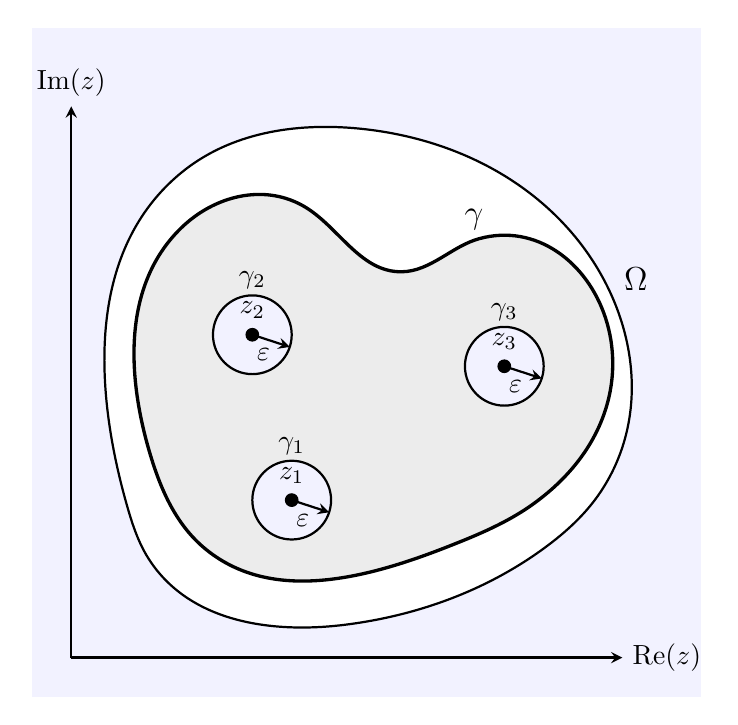
\begin{tikzpicture}
    \colorlet{GrayBackground}{gray!15}
    \tikzset{CircumferenceStyle/.style={draw=GrayBackground, ellipse, inner sep=0, fill=GrayBackground, name=EndVectorNode, above=0.02cm}}

    
    \colorlet{BlueBackground}{blue!5}
    % Background for entire canvas
    \fill[BlueBackground] (-0.5,-0.5) rectangle (8,8);
    \pgfmathsetmacro{\CircleSize}{0.08}     % radius of coordinate circles/dots
    % define styles used in this picture
    \tikzset{
    BigTextFont/.style={font=\large},
    every node/.style={font=\normalsize, text=black},
    CircleNodeStyle/.style={draw=black, shape=circle, fill=black, minimum size=\CircleSize*2 cm, inner sep=0pt},
    arrowstyle/.style={->, >=stealth}}

    % Axes
    \draw[thick, arrowstyle] (0,0) -- (0,7) node[above]{$\mathrm{Im}(z)$};
    \draw[thick, arrowstyle] (0,0) -- (7,0) node[right]{$\mathrm{Re}(z)$};
    
    % waypoint coordinates (in degrees, as seen from origin) for the two domains (in capital and small letters)
    \begin{scope}[scale=1.4]
    \coordinate (OD) at (4.3,1);
    \coordinate (20D) at (4.8,1.5);
    \coordinate (40D) at (4.5,3.9);
    \coordinate (55D) at (2.6,4.8);
    \coordinate (80D) at (1.0,4.4);
    \coordinate (110D) at (0.5,1.4);
    \coordinate (300D) at (0.7,0.9);
    \coordinate (330D) at (2.5,0.3);
    \end{scope}
    \begin{scope}[scale=1.4]
    \coordinate (Od) at (4.2,1.4);
    \coordinate (20d) at (3.7,3.8);
    \coordinate (40d) at (3.0,3.5);
    \coordinate (55d) at (2.1,4.1);
    \coordinate (80d) at (1.0,3.9);
    \coordinate (110d) at (0.7,1.9);
    \coordinate (300d) at (1.2,1.0);
    \coordinate (330d) at (3.4,1.0);
    \end{scope}
    
    
    % CHECK
    %plotting the waypoints
    %\foreach \c in {(Odegrees),(20degrees),(40degrees),(55degrees),(80degrees),
    %(95degrees),(110degrees),(180degrees),(260degrees),(300degrees),(330degrees)} \fill[red] \c circle (1.0mm);
    
    % center of epsilon area
    \coordinate (aLocation) at (2.8,2.0);   
    \node [CircleNodeStyle, label=above:$z_1$] at (aLocation) {};
    \coordinate (bLocation) at (2.3,4.1);   
    \node [CircleNodeStyle, label=above:$z_2$] at (bLocation) {};
    \coordinate (cLocation) at (5.5,3.7);   
    \node [CircleNodeStyle, label=above:$z_3$] at (cLocation) {};
    \coordinate (K) at (4,3);
    \node[above right] at (K) {$K$};
    
    \begin{scope}
        \clip[overlay] (aLocation) circle [radius=0.5]
        (-20,-20) rectangle (30,20);
        % fill in the areas with different colors
        \fill[white] (OD) to[closed, curve through ={(20D) (40D) (55D) (80D) (110D) (300D) }] (330D);
        \fill[GrayBackground] (Od) to[closed, curve through ={(20d) (40d) (55d) (80d) (110d)  (300d) }] (330d);
        \fill[BlueBackground] (aLocation) circle [radius=0.5];
        \fill[BlueBackground] (bLocation) circle [radius=0.5];
        \fill[BlueBackground] (cLocation) circle [radius=0.5];
    \end{scope}
    % drawing area ("hobby" package)
    \draw[postaction={decorate}, decoration={
           markings,
           mark=at position 0.17 with {\node[above right, BigTextFont] {$\Omega$};}}]
    [thick] (OD) to[closed, curve through =
    {(20D) (40D) (55D) (80D) (110D) (300D) }] (330D);
    % drawing area ("hobby" package)
    \draw[postaction={decorate}, decoration={
           markings,
           mark=at position 0.27 with {\node[above, BigTextFont] {$\gamma$};}}]
    [very thick] (Od) to[closed, curve through =
    {(20d) (40d) (55d) (80d) (110d) (300d) }] (330d);

    \node [CircleNodeStyle, label=above:$z_2$] at (bLocation) {};
    \node [CircleNodeStyle, label=above:$z_3$] at (cLocation) {};
    
    % create epsilon area
    \draw[thick] 
    [postaction={decorate}, decoration={
           markings,
           mark=at position 0.25 with {\node[CircumferenceStyle] {$\gamma_1$};},    % ensure node has a white background
           mark=at position 0.95 with {\node[name=EndVectorNode] {};}}]
    (aLocation) circle [radius=0.5];
    
    % draw radius of area
    \draw[thick, arrowstyle]
    [postaction={decorate}, decoration={
           markings,
           mark=at position 0.3 with {\node[name=EndVectorNode, below] {$\varepsilon$};}}] 
    (aLocation) -- (EndVectorNode.center);
    % create epsilon area
    \draw[thick] 
    [postaction={decorate}, decoration={
           markings,
           mark=at position 0.25 with {\node[CircumferenceStyle] {$\gamma_2$};},    % ensure node has a white background
           mark=at position 0.95 with {\node[name=EndVectorNode] {};}}]
    (bLocation) circle [radius=0.5];
    
    % draw radius of area
    \draw[thick, arrowstyle]
    [postaction={decorate}, decoration={
           markings,
           mark=at position 0.3 with {\node[name=EndVectorNode, below] {$\varepsilon$};}}] 
    (bLocation) -- (EndVectorNode.center);
    % create epsilon area
    \draw[thick] 
    [postaction={decorate}, decoration={
           markings,
           mark=at position 0.25 with {\node[CircumferenceStyle] {$\gamma_3$};},    % ensure node has a white background
           mark=at position 0.95 with {\node[name=EndVectorNode] {};}}]
    (cLocation) circle [radius=0.5];
    
    % draw radius of area
    \draw[thick, arrowstyle]
    [postaction={decorate}, decoration={
           markings,
           mark=at position 0.3 with {\node[name=EndVectorNode, below] {$\varepsilon$};}}] 
    (cLocation) -- (EndVectorNode.center);

\end{tikzpicture}

\end{document}